% \iffalse
% <*SPECIALS>
% \fi
% \cxset{chapter beforeskip   = 0pt,
%        chapter afterskip=0pt,  
%       }
%
% \chapter{Custom Formatters}
%
% \normalsize
% Now what happens, if none of the formats can adequately describe a heading? 
% How can we define a mark-up language for more complex layoutS.
% The way proposed here is to use the formatter methods coded earlier.
% So far all the formatters we have programmed used only textual elements. 
% Many complex designs for headings incorporate images as well as additional
% subtitles and even mini-table of contents.
%
% To create a new format we need to code a templating command as well as create a set
% of additional keys to cater for any component of the heading that is not adequately
% covered by the generic keys.
%
% As a convention each special format has a unique name. For example the |stewart| format
% has an associated control sequence |stewart| and the one shown in this heading
% is called |fashion|, as it started as such although I was tempted to name
% it euro! Most of the additional templates provided by the \pkg{phd} package use
% \tikzname to render their output. This is not always necessary and any valid \tex code
% can be used for templates.
%
% I have kept to the convention that values for all keys should be in lower case and hence
% function names must follow suit.
%
%  \cxset{chapter format=stewart,
%         section format = hang}
%
% \chapter{The stewart template}
%
% The stewart template has been named after \emph{Stewart's Calculus}, where a similar design
% gave me the inspiration. It uses an image as well as banded notes and comments. It is
% ideal for textbooks, when used to render chapter heads. 
%
% Start by defining some additional keys:
%
%    \begin{macrocode}
\ExplSyntaxOn
\cxset{
    offsety/.store~in        = \soffsety,
    image/.store~in          = \image@cx,
    texti/.store~in          = \texti@cx,
    textii/.store~in         = \textii@cx,
}

\cxset{offsety = 0pt,
       image   = hine02,
       texti   = \lorem,
       textii  = \lorem }    
\cxset
  {
    steward/.style = {
    offsety/.store~in        = \soffsety,
    image/.store~in          = \image@cx,
    texti/.store~in          = \texti@cx,
    textii/.store~in         = \textii@cx,
    %chapter~beforeskip       = 1sp,
    %chapter~afterskip        = 1sp,
  }
}

\ExplSyntaxOff
%    \end{macrocode}
% 
\cxset{stewart, image=hine02}
% \begin{docCommand} {stewart} { \marg{element name} \marg{title} }
%   Special formatter to style headings on a full page. 
% \end{docCommand}

%    \begin{macrocode}
\ExplSyntaxOn
\newcommand\stewart[2]
  {
    \clearpage
    \thispagestyle{empty}
    \begin{tikzpicture}[remember~picture,overlay]
      \node [xshift=5cm,yshift=-\paperheight] at (current~page.north~west)
            [
              text~width=\textwidth-1cm,
              text~height=\paperheight, 
              fill=thecream!30,
              rounded~corners,
              above~right
            ]
            {};
            
      \node [xshift=6.5cm,yshift=-1.5cm-\soffsety] at (current~page.north~west)
            [text~width=0.7\textwidth,below~right]
            {
             \language-1
             \sffamily \bfseries \huge #2
            };

     \node [xshift=3cm,yshift=-1.5cm] at (current~page.north~west)
           [
             text~width=3cm,
             align=center,
             minimum~height=2.5cm, 
             fill= thechaptercolor,
             below~right]
           {
           
             \text{\HHUGE\bfseries\sffamily\color{white}
             \cs:w the#1 \cs_end:}
              
             \par\vspace*{3pt}
           };

     \node [xshift=-0.2cm,yshift=-21.5cm] at (current~page.north~west)
           [text~width=3cm,above~right]%
           {\includegraphics[width=1.0\paperwidth,
             height=\textheight,keepaspectratio]{\image@cx}};
     
     \node [xshift=3cm,yshift=-19.5cm] at (current~page.north~west)
           [text~width=9cm,minimum~height=2.5cm,
           inner~sep=0.5em, 
           fill= thechaptercolor,
           below~right]
           {\color{white}
            \bfseries\sffamily\texti@cx
           };

     \node [xshift=5.5cm,yshift=-26cm] at (current~page.north~west)
           [text~width=10cm,above~right]
           {
             \textii@cx 
           };
\end{tikzpicture}
\ExplSyntaxOff
%    \end{macrocode}
% Since we are using an overlay, there is no bounding box, hence we need
% to issue a \cs{clearpage} explicitly.
%    \begin{macrocode}
\par
\clearpage
\ExplSyntaxOn

\phd_after_heading:
\ExplSyntaxOff
}
%    \end{macrocode}
%
% \section{An interesting template}
%
% Many books, especially those rich in images tend to have main heading openings
% with photo spreads. The following template code does this.
%
%    \begin{macrocode}
\ExplSyntaxOn
\newcommand\hdr[2]
  {
    \clearpage
    \thispagestyle{empty}
    \begin{tikzpicture}[remember~picture,overlay]
    \node [xshift=-12cm,yshift=3pt] at (current~page.north~west)
           [below~right,
            minimum~height=\paperheight]
           {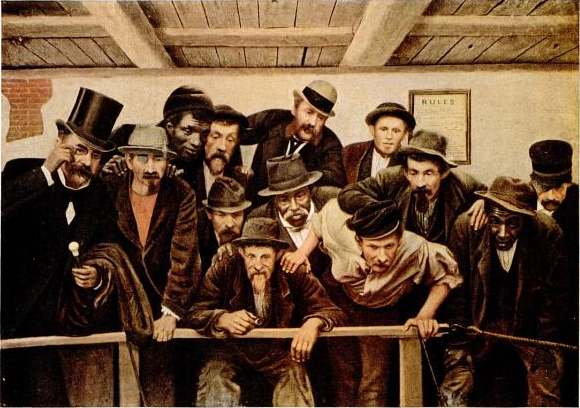
\includegraphics[
             height=\paperheight]{cockfight}}; 
    \end{tikzpicture}
    
    \clearpage 
    \thispagestyle{empty}        
    \begin{tikzpicture}[remember~picture,overlay]
         
      \node [xshift=0cm,yshift=0] at (current~page.north~east)
           [
             text~width=3.5cm,
             align=center,
             minimum~height=2.5cm, 
             fill=bgsexy,
             below~left]
           {
           
             \text{\HHUGE\bfseries\sffamily\color{white}
             \cs:w the#1 \cs_end: }
             \par\vspace*{3pt}
           };
           
\node [xshift=-2.7cm,yshift=-10pt] at (current~page.north~east)
           [
             below~right,rotate=-90]
           {
           
             {\footnotesize\bfseries\sffamily\color{white}
             \expandafter\MakeTextUppercase{\cs:w #1name \cs_end:}
             }
             \par\vspace*{3pt}
           };
           
\node [xshift=-1.2cm, yshift=-3cm] at (current~page.north~east)
           [
             below~right,rotate=-90]
           {
           
             {\Huge\bfseries\sffamily\cs_if_exist_use:c {the_chapter_title_fontface_tl}
              \color{bgsexy}
             \MakeTextUppercase{#2}
             }
             \par\vspace*{3pt}
           };
           
\node [xshift=-\paperwidth-9cm,yshift=3pt] at (current~page.north~west)
           [below~left]%
           {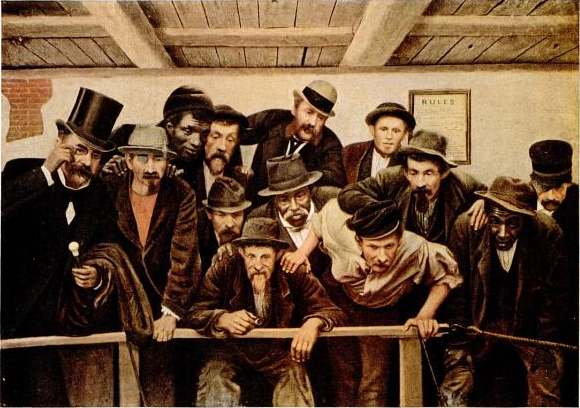
\includegraphics[
             height=\paperheight]{cockfight}};           
           
\end{tikzpicture}
\ExplSyntaxOff
%    \end{macrocode}
% Since we are using an overlay, there is no bounding box, hence we need
% to issue a \cs{clearpage} explicitly.
%    \begin{macrocode}
\par
\newpage
}
%    \end{macrocode}


%    \begin{macrocode}
\def\soffsety{2pt}
\def\image@cx{hine01}
\def\texti@cx{\lorem}
\def\textii@cx{\lorem}
%    \end{macrocode}

%    \begin{macrocode}
\newcommand\stewartpart[1] {%
% need an additional clear as it is picture, overlay, otherwise text comes in
% from the next page.

 \clearpage

\begin{tikzpicture}[remember picture,overlay]
\node [xshift=5cm,
       yshift=-\paperheight] at (current page.north west)
      [text width=0.99\textwidth,
      text height=\paperheight, 
      fill=thecream!30,
      above right]
{};
% set title
\node [xshift=8.5cm,yshift=-1.5cm-\soffsety] at (current page.north west)
[text width=0.9\textwidth,below right]{\sffamily \bfseries \HUGE \thechapter};
% set part
\node [xshift=4cm,yshift=-1.5cm] at (current page.north west)
[text width=4cm,align=center,minimum height=2.5cm, fill=blue,below right]
{\color{white}\bfseries\sffamily \MakeTextUppercase{#1}
\\ \text{\HHUGE\@Roman\c@part\relax}
};
% photograph
\node [xshift=-0.2cm,yshift=-21.5cm] at (current page.north west)
[text width=3cm,above right]%
{\includegraphics[width=1.0\paperwidth,height=\textheight,keepaspectratio]{\image@cx}};
\node [xshift=3cm,yshift=-19.5cm] at (current page.north west)
[text width=9cm,minimum height=2.5cm,inner sep=0.5em, fill=blue,below right]
{\color{white}
  \bfseries\sffamily\texti@cx
};
\node [xshift=6.5cm,yshift=-26cm] at (current page.north west)
[text width=12cm,above right]
{\textii@cx
};
\end{tikzpicture}
\par
\clearpage
}
%    \end{macrocode}
%
% \subsection{tikzspecials}
%    \begin{macrocode}
\ExplSyntaxOn
\cxset{band~height/.store~in=\bandheight@cx}
\cxset{band~height=5cm}

\newcommand{\tikzspecial}[1]{%

\clearpage
\ExplSyntaxOn
\let\titlefontfamily@cx\l_phd_title_font_family_tl
\let\titlefontweight@cx\l_phd_title_font_weight_tl
\ExplSyntaxOff

\begin{tikzpicture}[remember~picture,overlay]
    \node[yshift=-\bandheight@cx]~ at~ (current~page.north~west)
      {\begin{tikzpicture}[remember~picture, overlay]
        \draw[fill=bgsexy, draw=none] (0,0) rectangle (\paperwidth,\bandheight@cx);
        \node[anchor=east,
              xshift=.9\paperwidth,
              rectangle,
              rounded~corners=10pt,inner~sep=11pt,
              text~width = 0.7\linewidth,
              fill=black!80]{%
%        \titlefontcolor@cx
%        title_font_size
          \LARGE
          \bfseries
          \sffamily
%        \titlefontfamily@cx
             \lineskip2pt
             \color{white}
             \thechapter\
             \textsc{#1}};
       \end{tikzpicture}
      };
\end{tikzpicture}
\mbox{}
\vspace*{\bandheight@cx}\par
\phd_after_heading:
}
\ExplSyntaxOff
%    \end{macrocode}
%
% \section{The genetics special design}
%
%    \begin{macrocode}
\cxset{image/.store in=\image@cx,
       image caption/.store in=\caption@cx,
       textiii/.store in=\textiii@cx}
\cxset{image      = genetics-dogs,
       image caption = Genetics,
       textiii       = \lorem}       
%    \end{macrocode}
%
% 
%	This macro is a special template that requires settings via
%	a |\cxset| command. 
%    \begin{macrocode}
\ExplSyntaxOn
\newcommand\genetics[1]{%
  %    \end{macrocode}
% 
%
%	We set everything in a minipage to ensure that no breaks will
%	occur. If the user added too much text it will just overflow and it
%	will have to be adjusted.
%    \begin{macrocode}
\begin{minipage}[b][\textheight][t]{\textwidth}%
\hbox{}%
%    \end{macrocode}
%	We first draw the rules.
%    \begin{macrocode}
      \vbox to 0pt {%
      \color{teal}%
      \hbox{\rule{\textwidth}{0.4pt}}%
      \hbox{\rule{0.4pt}{\textheight}\rule{4cm}{0.4pt}}%
    }%
\vspace*{10pt}%
%    \end{macrocode}
%	The next two parboxes, place the subtitle and the image.
% 	they are aligned at the bottom and a rule can be used to adjust the 
%	subtitle.
%
%    \begin{macrocode} 
\begin{minipage}[b]{\linewidth}%
\fboxsep0pt%
\fboxrule0pt%
\fbox{\begin{minipage}[b]{0.25\linewidth}%
\lineskip0pt\topskip0pt%
\leftskip0.5cm%
\leavevmode%
\bfseries\color{teal}\Large\sffamily%
\caption@cx%
\vspace*{2cm}%
\par
\includegraphics[width=\dimexpr\linewidth-0.5cm\relax,totalheight=3.8cm]{./images/chapterconcept-01.jpg}\llap{\raise20pt\hbox to \linewidth{\HHUGE \hskip1cm\color{lightgray!40}\thechapter}\hfill}%
\end{minipage}%
}%
%
\fbox{\begin{minipage}[b]{0.75\linewidth}%
\lineskip0pt%
\leavevmode
\includegraphics[width=1\linewidth]{\image@cx}%

\includegraphics[width=\linewidth]{./images/chapterconcept-02.jpg}.%
\end{minipage}}%
\end{minipage}%
%    \end{macrocode}
%    \begin{macrocode}
\par
\vspace{1.5cm  plus25pt minus25pt}
\parbox[t]{0.3\linewidth}{%
  \set_font_aux:n {l_phd_chapter}
  \leftskip0.5em 
  \color{teal}#1%
}%
\begin{minipage}[t]{0.6\linewidth}%
\vspace{-2\baselineskip}
\textiii@cx
\end{minipage}

\end{minipage}
\markboth{#1}{#1}
}
\ExplSyntaxOff
%    \end{macrocode}
%
% \cxset{chapter format=fashion,}
% \definecolor{thechaptercolor}{HTML}{140F15}
% \long\def\storyi{A formatter that can be used both for sections or chapters. It is a more modern
%  design with a photo. It has a similarity to the \textit{andrea} template. The template interacts 
% with the colorpalette in a minimal way to provide a touch of color to
% the number box and the title. It uses additional positional keys and subtitle keys. One limitation is that the subtitle text needs to be about right in relation to the photo on the right. By default it does not typeset the chapter or section label. It has exactly the same design both for verso and recto pages.}
%
% \chapter*{The Fashion Template}
%
% \section*{Introduction}
%
% \section{Introduction no star no value}
%
% \tcbdocmarginnote{R 2019/01/29}
% \noindent The inspiration for this was from a fashion magazine. I ended up with the gridlines that were 
% used  for testing, but I liked them and left in permanently.
%
% The template interacts with the colorpalette in a minimal way to provide a touch of color to
% the number box and the title. The background of the box uses the |thechaptercolor|. The same color
% is used to typset the title. 
%
% The width of the block is 16cm and the height takes almost the full textblock $\pm$~18cm. 
% 
% \begin{docCommand} {fashion} {\meta{*} \Arg{element name} \Arg{title text} \hfill\hfill \Arg{a,b,c,d} }
% \end{docCommand}
%
%
%    \begin{macrocode}
%<@@=fashion>
%    \end{macrocode}
% \paragraph{Additional keys for the template}
% Add some additional keys for the template. These handle image dimensions and the bylines.
%    \begin{macrocode}
\ExplSyntaxOn
\cxset{
  fashion~image/.code            = \cs_set:Npn \l_@@_image {#1},
  subtitle~font-color/.store~in  = \@@_subtitlefontcolor,
  fashion~image~width/.code      = \cs_set_nopar:Npx \@@_image_width {#1},
}
% set default image
\cxset
  {
    fashion~image                = fashion-02.jpg,
    subtitle~font-color          = black!95,
    fashion~image~width          = 5cm,
  }
\ExplSyntaxOff
%    \end{macrocode}
%

%default value for the image width    
%    \begin{macrocode}
\ExplSyntaxOn
\def\fashionnumberbg {gray!30}
\@debugtrue
\if@debug
   \tikzset{fashion/.style = rectangle, draw}
\else   
\fi
\ExplSyntaxOff

\DeclareDocumentCommand \storyi {} 
{
  In antiquity men and women saw each other as different; 
  accordingly, they developed
  complex taxonomies (philosophical explanations) 
  for understanding anatomical,
  physiological, emotional, and rational differences. \par

  Some of these differences seem profoundly odd to us moderns. 
  Modern discussions about erotic art have often concerned 
  the place of women: to what
  extent are they objects of social manipulation, to what 
  extent can they be subjects?
}
\ExplSyntaxOn
\dim_new:N \fashionwidth_dim
\dim_new:N \fashionwidth_height
\newif\if@hasstar

\DeclareDocumentCommand\fashion {s m m}
  { 
    \IfBooleanTF {#1}
      {\fashion_aux:nn {#2} {#3} {\global\@hasstartrue}  }
      {\fashion_aux:nn {#2} {#3} {\global\@hasstarfalse} }
  }
  
\cs_set:Npn \fashion_aux:nn #1 #2 #3{%
%    \end{macrocode}
% Since this is a template recommended for full page display, we do not use
% absolute positioning with |remember, picture overlay| but rather measure and 
% shift as necessary.
%
%    \begin{macrocode}
  \dim_set:Nn \fashionwidth_dim {16cm}
 
  
   \dim_set:Nn \l_tmpa_dim {0pt}
   
   % need to shift to the left
   \ifdim\linewidth < \fashionwidth_dim
    \dim_set:Nn \l_tmpa_dim {(\fashionwidth_dim-\pagewidth)/2}
   \else
    \dim_set:Nn \l_tmpa_dim {0pt} 
   \fi
%    \end{macrocode}
% Use \docAuxEnvironment{adjustwidth} from the \pkg{changepage} to adjust the margins. 
% Note that the environment uses a |\list|.
%    \begin{macrocode}   
 \begin{adjustwidth}{-2.1cm}{2.00002cm}
 \parindent0pt
   \begin{tikzpicture}[yshift=-5cm]
  \if@debug 
    % helplines grid(x,y)
    \draw [help~lines,color=black!10] (0,0) grid (\fashionwidth_dim+1cm,-18);
    \foreach \y in {0,...,18}{%
    
    \draw[fill=black]  (\linewidth+\rightmargin-\leftmargin+4.5pt,-\y) circle (.5pt) ++(7pt,0) node {{\tiny-\y}};} ;
  \else
  \fi
  % draw debug rectangles
  \node[fashion, right, baseline] (x) at (0,1) {\LARGE\color{black!30}{}\relax};
  %\draw[fill=red]  (0,1) circle (1.5pt) ;
  \node[fashion, right=1sp] at (0,-1) 
    {
      {\LARGE\color{the#1color} \cs:w chaptername\cs_end:\relax} 
    };
%    \end{macrocode}
%
% Check if we need to print the number or not and act accordingly.
%    \begin{macrocode}
#3
\if@hasstar
\else
 
  \node[rectangle,draw, 
      color = thechaptercolor, 
      below~left, 
      drop~shadow,
      fill= thechaptercolor, 
      text=white,
      ] at +(15,-0.5) {\HHUGE\sffamily\bfseries\color{white}\thechapter};
\fi      
%    \end{macrocode}
%
% Next add the section title and byline
%    \begin{macrocode}
\node[fashion, text~width=9cm,below~right, yshift=-1pt] at (0,-3) 
  {%
        {%
          \sffamily\RaggedRight
          %dis-allow hyphenation 
          \language-1
          \Huge\bfseries\color{thechaptercolor}#2\par}
           \bigskip
           \Large% 
           \centering
           \color{\@@_subtitlefontcolor 
         }%
%    \end{macrocode}
%
% Add the story lines. These are entered separately bey defining a macro |\storyi|
%    \begin{macrocode}
        \storyi
        
        %\dim_use:N \fashionwidth_dim
        {\small
        \dim_to_decimal_in_unit:nn  {\the\pagewidth  }{1cm }\par
        \dim_to_decimal_in_unit:nn  {\dim_use:N \fashionwidth_dim}{1cm}\par
        \dim_to_decimal_in_unit:nn  {\dim_use:N \l_tmpa_dim}{1cm}\par
        \dim_to_decimal_in_unit:nn  {\dim_use:N \leftmargin}{1cm}\par
         \dim_to_decimal_in_unit:nn  {\dim_use:N \leftmargini}{1cm}\par
        }
        \par
  }; 
% Add the image        
        \IfFileExists{./images/\l_@@_image}   
           {\node[below~left,
                  outer~sep=0pt,
                  inner~sep=0pt,
                  drop~shadow = {
                  shadow~scale=1.0, 
                  shadow~xshift=50pt,
                  shadow~yshift=-10pt,
                  fill=white,
                  opacity=0.2},
                  rounded~corners,yshift=2cm,
                  ] at (14.5,-10.5) {\includegraphics[width=\@@_image_width]{\l_@@_image}};}%
           {\node at (12.5,-10.5) {\includegraphics[width=5cm]{./images/venus}};}%
\end{tikzpicture}
\end{adjustwidth}
\thispagestyle{plain}
\vfill
\newpage
}
\ExplSyntaxOff
%    \end{macrocode}

% This template was developed before the \pkg{xcoffins} package had the current stability. It can benefit
% to using coffins to position the image relative to the text.
%
% - Some cropping of the image maybe necessary.
%
% - Should have a draft function for speed?
%
% - Change tikz keys to fashion style, as a programmer API.
%
% Star version of the command?
%
% </SPECIALS>
\endinput
